\chapter{Test dell’\textit{edge-recommendation system} in modalità \textit{greedy e non}}
\label{chap:test}

Il sistema implementato è stato sottoposto a vari test con lo scopo di valutare i due algoritmi di \textit{k-edge recommendation} alternativi, ovvero \textit{greedy e non greedy}, ed in modo tale da poterli confrontare tra loro in termini di:
\begin{itemize} 
\item decremento totale dell'\textit{RWC} che ciascuno di essi consente di apportare ad un certo \textit{retweet graph} in input, a parità di numero di archi proposti \textit{k};
\item qualità dei \textit{k} archi scelti, in termini del \textit{$\delta RWC$} associato a ciascuno di essi;
\item tempi di esecuzione.
\end{itemize}

I \textit{retweet graphs} utilizzati come input dei test corrispondono alle discussioni attorno agli \textit{hashtags} controversi \textit{\#beefban, \#indiana, \#russia\_march}, le cui informazioni (i.e. \textit{tweets} e \textit{retweets} emessi nel periodo di osservazione) sono reperibili presso il \textit{repository} degli autori dell'articolo \cite{garimella:paper}. Pertanto, in questo caso, non è stato necessario eseguire il \textit{processo di raccolta dati} descritto nel capitolo precedente ma, per ciascuno degli \textit{hashtags} appena menzionati, è bastato \textit{parsare} il relativo file dei \textit{retweets} (disponibile nel \textit{repository}) e creare il \textit{retweet graph} corrispondente.
\\I \textit{retweet graphs} creati, relativi agli \textit{hashtags} di cui sopra, hanno le seguenti caratteristiche:
\\\\
\begin{tabular}{l*{6}{c}r}
\textbf{Hashtag}         & \textbf{|V|} & \textbf{|E|}  \\
\hline
\#beefban 		 & 1610 & 1978  \\
\#indiana        	 & 2467 & 3143  \\
\#russia\_march   	 & 2134 & 2951  \\
\end{tabular}
\\\\\\
I parametri del sistema sono stati impostati con i seguenti valori:
\begin{itemize}
\item $\alpha = 0.85$;
\item $k_1 = 20$; 
\item $k_2 = 20$;
\item $k = 50$.
\end{itemize}
Nel prossimo paragrafo, per ciascuno dei tre \textit{retweet graphs} in input, verranno mostrati e commentati i risultati dei test relativi alla discesa dell'\textit{RWC} ottenuta a seguito dell'applicazione di ciascuno dei due algoritmi di \textit{recommendation} proposti. 

\section{Discesa dell'\textit{RWC}}

Di seguito inseriamo i grafici che mostrano la discesa dell'\textit{RWC} dei \textit{retweet graphs} relativi agli \textit{hashtags} considerati, nell'ordine:
\begin{enumerate}
\item \textit{\#beefban};
\item \textit{\#indiana};
\item \textit{\#russia\_march}.
\end{enumerate}

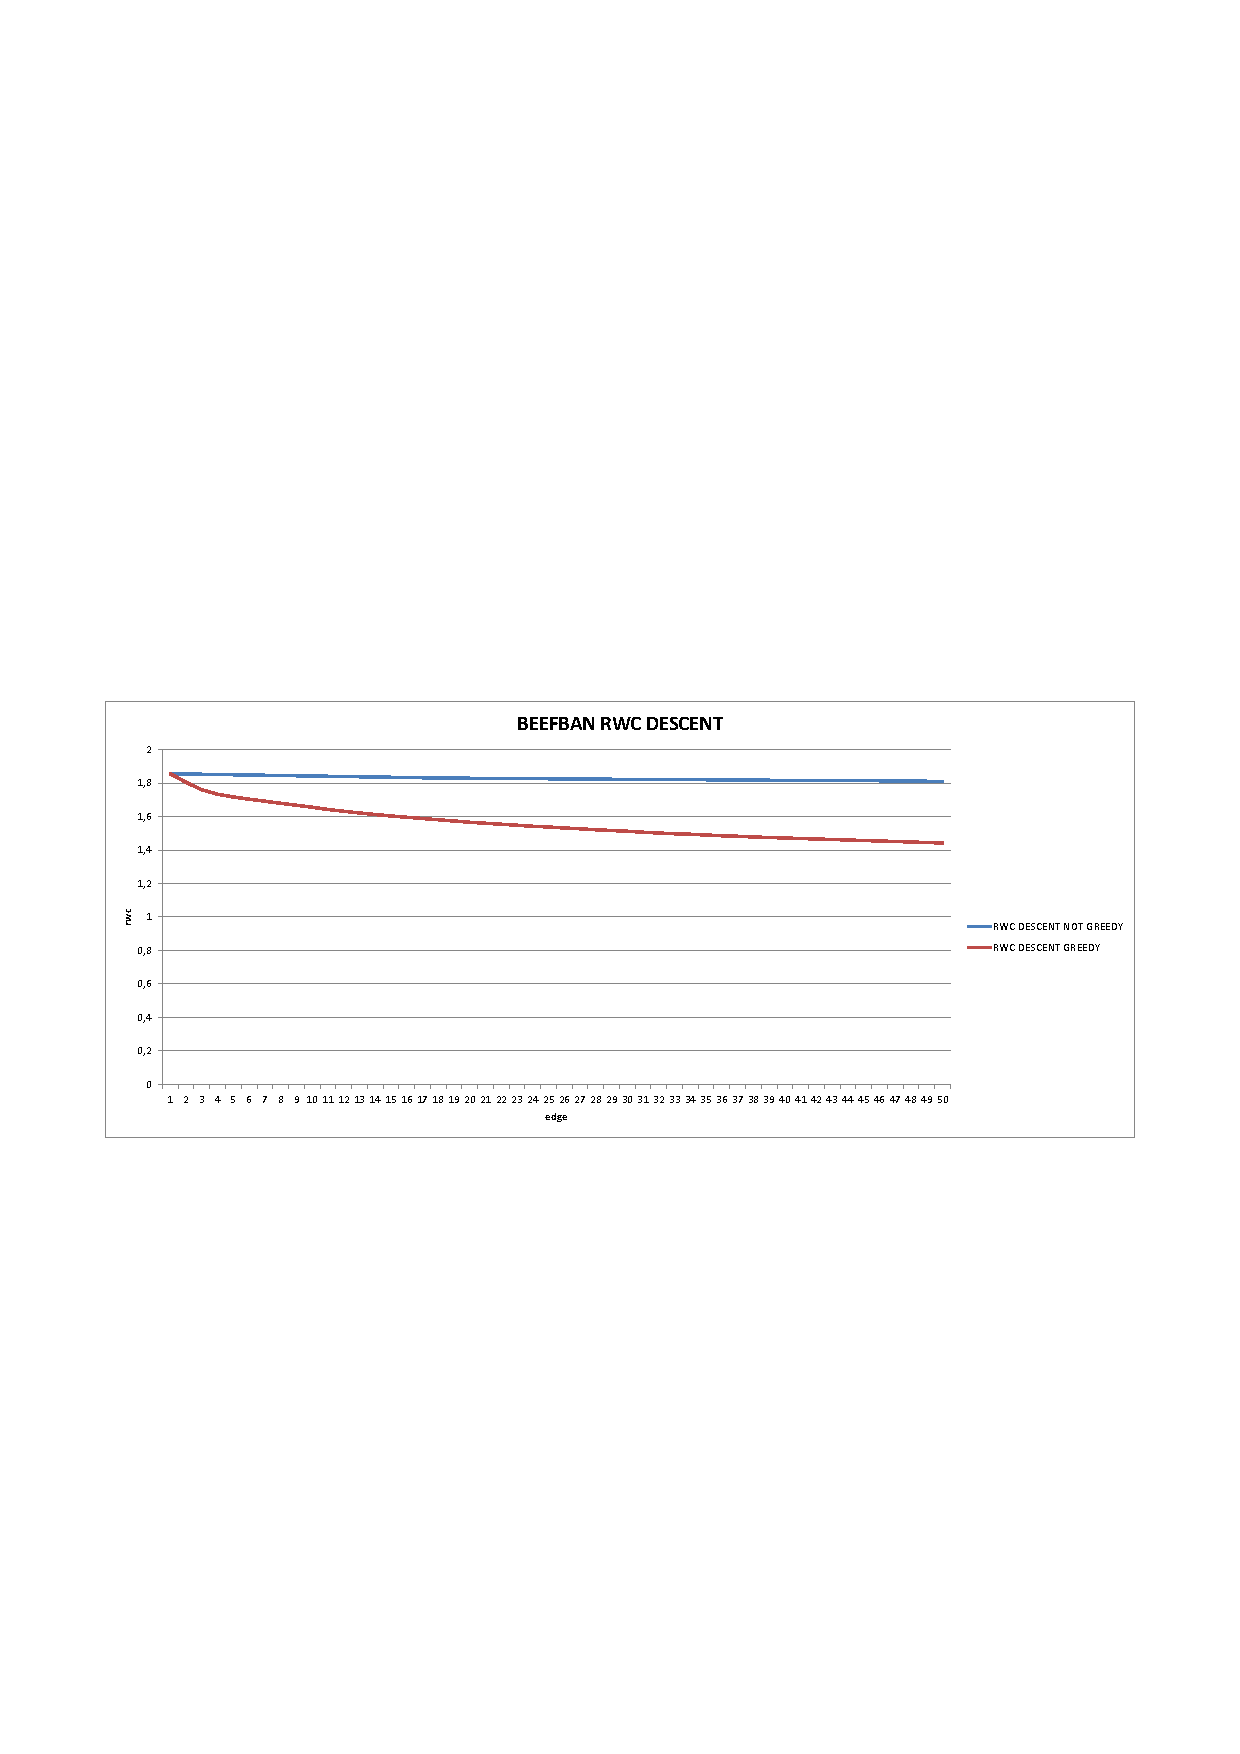
\includepdf{images/BEEFBAN_IN_DEG_PROBABILITY_FREE_RWC_DESCENT.pdf}
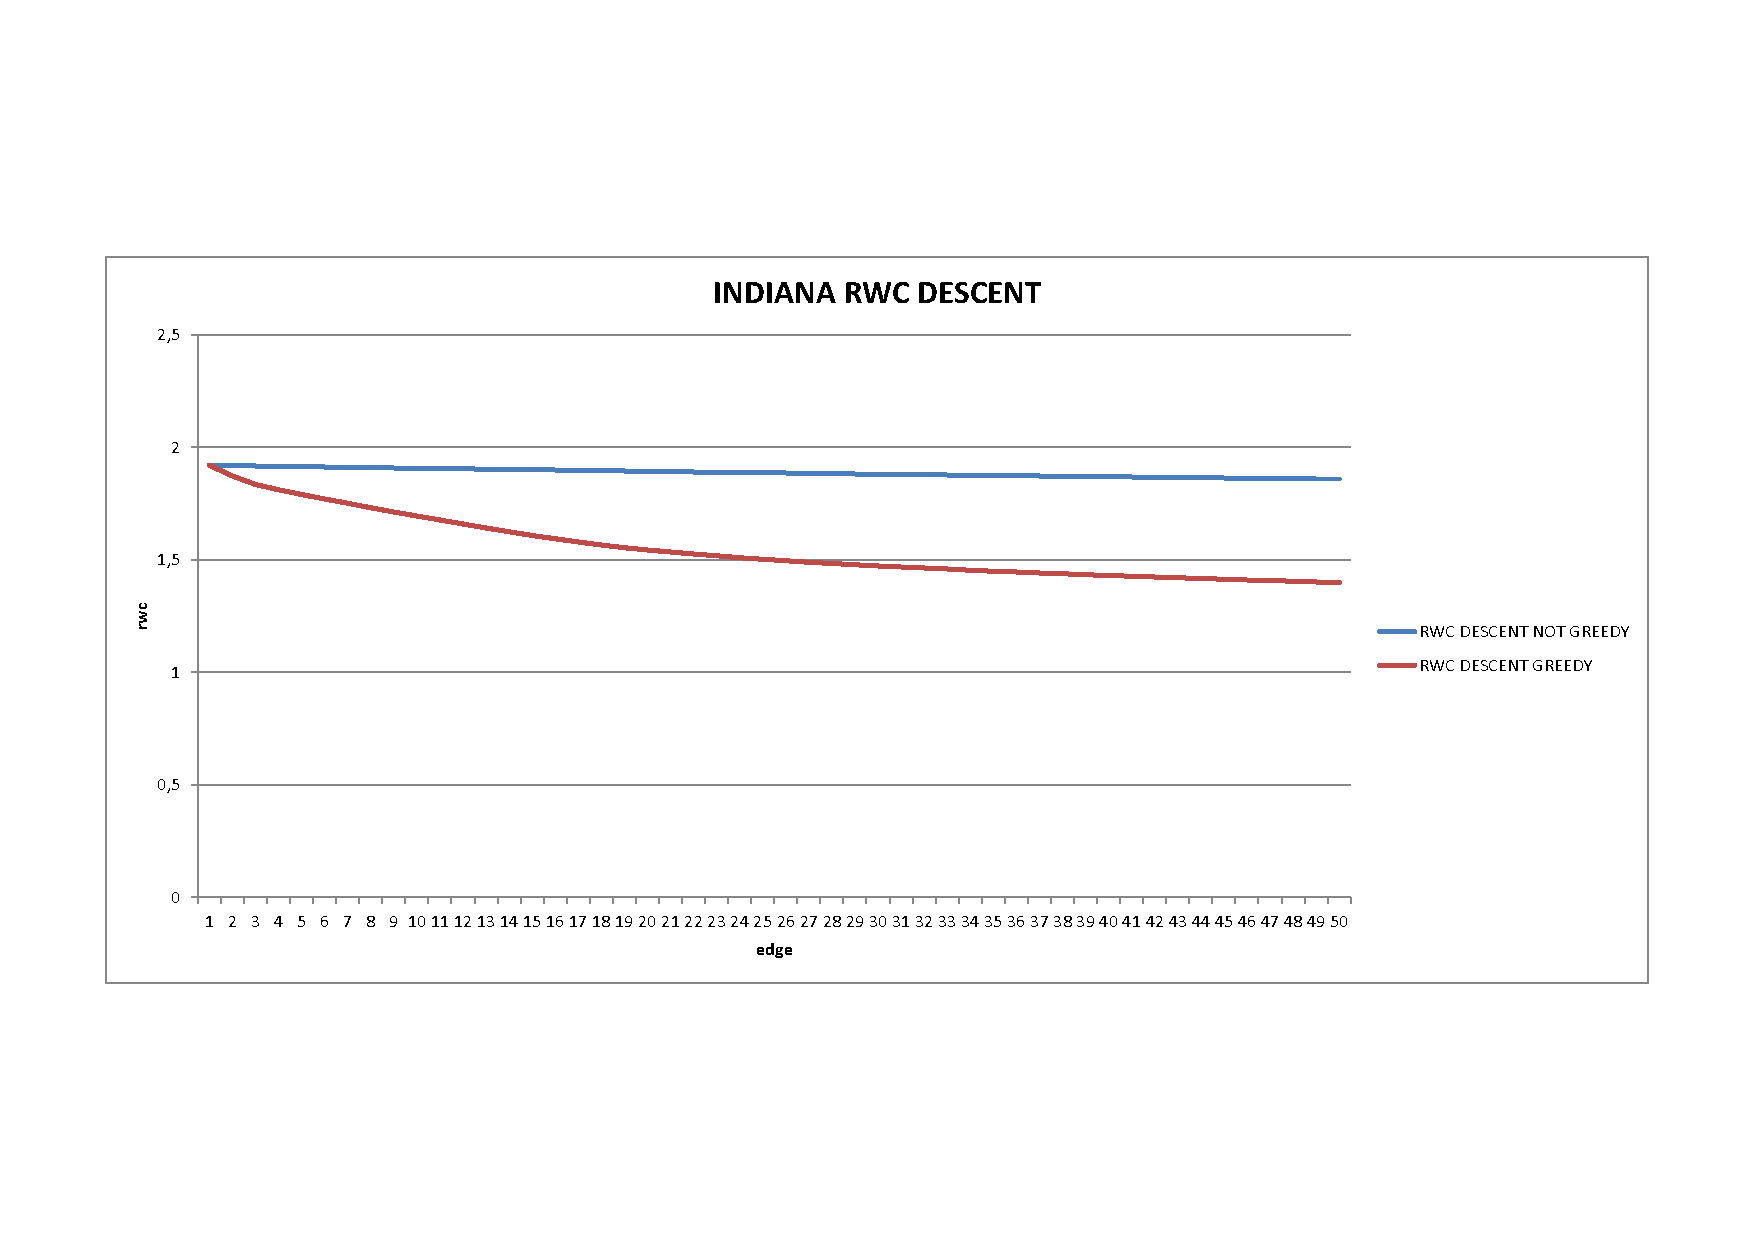
\includepdf{images/INDIANA_IN_DEG_PROBABILITY_FREE_RWC_DESCENT.pdf}
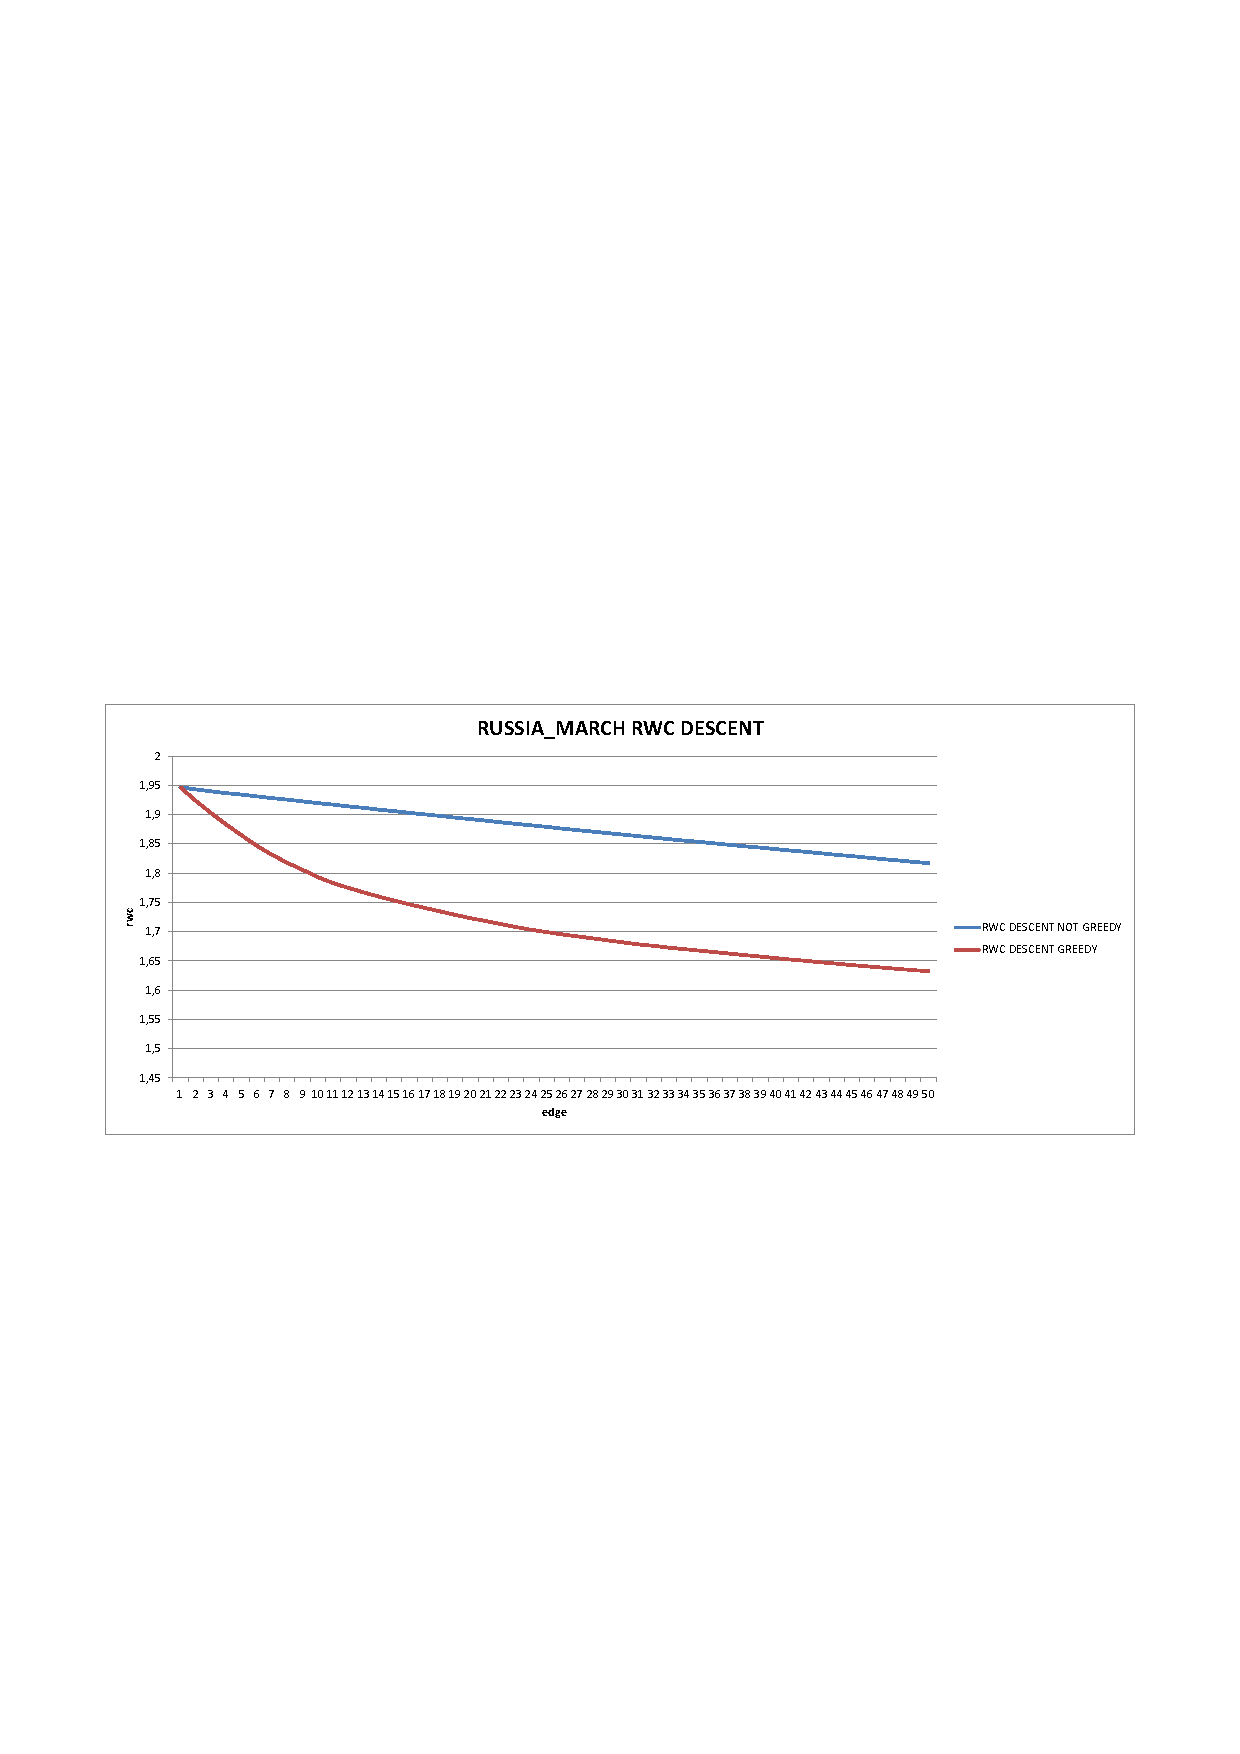
\includepdf{images/RUSSIA_MARCH_IN_DEG_PROBABILITY_FREE_RWC_DESCENT.pdf}
Ciascuno dei tre grafici, uno per \textit{retweet graph}, ha l'obiettivo di porre a confronto i decrementi dell'\textit{RWC} che rispettivamente i due algoritmi di \textit{edge recommendation} consentono di raggiungere a parità di archi proposti. 
\\In particolare, fissato un \textit{retweet graph g}, il grafico corrispondente mostra due funzioni, rispettivamente di colore \textit{rosso} e di colore \textit{blu}, con valori nel dominio \textit{$0 < j \leq k$}:
\begin{itemize}
\item \textit{RWC(g,j)\textsubscript{greedy}}, ovvero l'\textit{RWC} che caratterizzerebbe il \textit{retweet graph g} qualora i primi \textit{j} archi proposti dall'algoritmo \textit{greedy} si materializzassero nel grafo; 
\item \textit{RWC(g,j)\textsubscript{non-greedy}}, ovvero l'\textit{RWC} che caratterizzerebbe il \textit{retweet graph g} qualora i primi \textit{j} archi proposti dall'algoritmo \textit{non-greedy} si materializzassero nel grafo.
\end{itemize}
Come si nota immediatamente dai grafici, per ogni \textit{retweet graph g} considerato vale:
\\\\
$\textit{RWC(g,j)\textsubscript{greedy}} \leq \textit{RWC(g,j)\textsubscript{non-greedy}}, \forall j = 1,..,k$
\\\\
Ovvero, a parità di archi proposti, l'algoritmo \textit{greedy} consente \textit{sempre} di raggiungere un decremento dell'\textit{RWC} maggiore o uguale, per ciascun grafo \textit{g}. Questa maggiore \textit{efficacia} dell'algoritmo \textit{greedy} non soprende, viste la considerazioni e le analisi condotte nei capitoli precedenti, e deriva sostanzialmente dalla maggiore \textit{qualità}, in termini di decremento del \textit{grado di controversia}, di ciascun arco che propone. 
\\Il paragrafo a seguire si occuperà proprio di confrontare gli archi proposti dai due algoritmi \textit{greedy} e \textit{non-greedy}, in termini dei \textit{$\delta RWC$} corrispondenti.

\section{Qualità degli archi proposti}
Ognuno dei seguenti grafici, corrispondenti ai tre \textit{retweet graphs} considerati, associa ad ogni arco, proposto da ognuno dei due algoritmi, il relativo \textit{$\delta RWC$}.

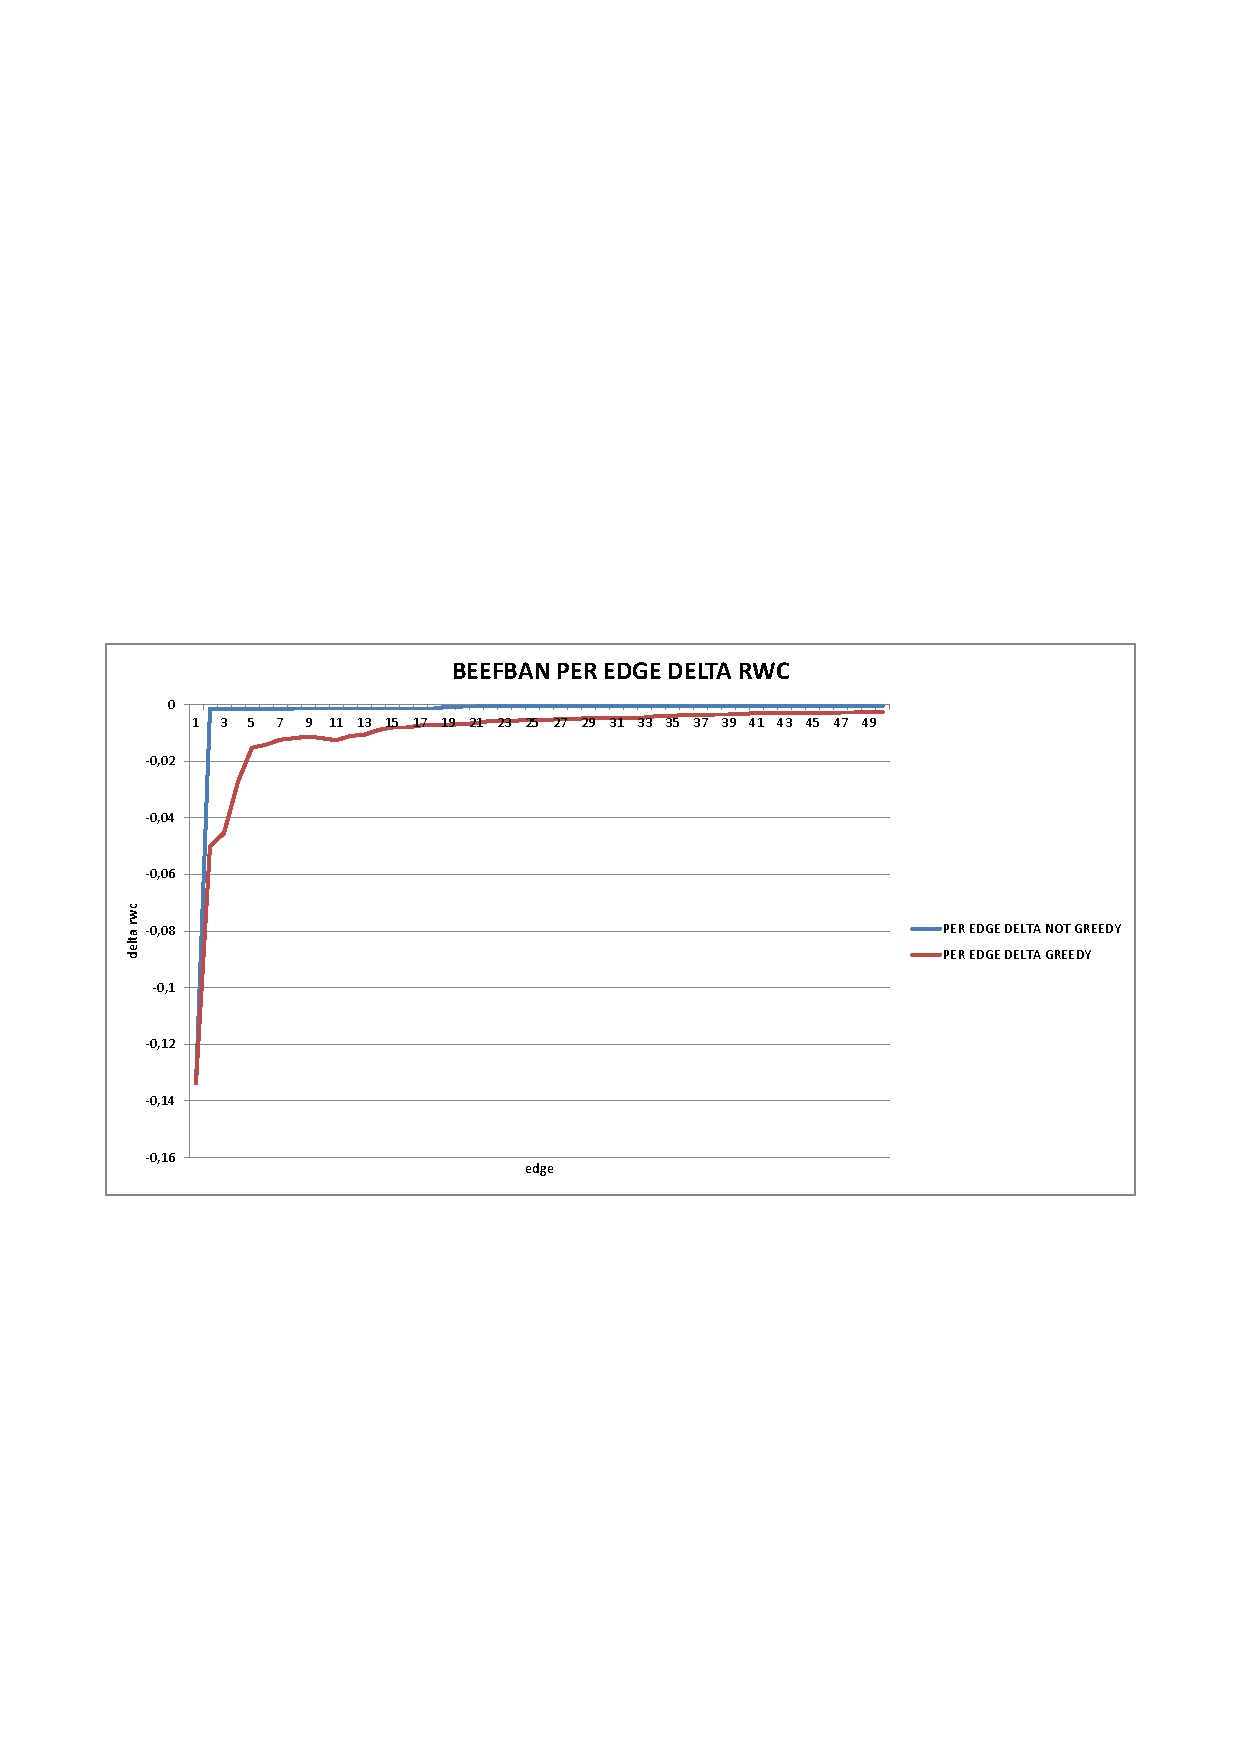
\includepdf{images/BEEFBAN_IN_DEG_PROBABILITY_FREE_PER_EDGE_DELTA.pdf}
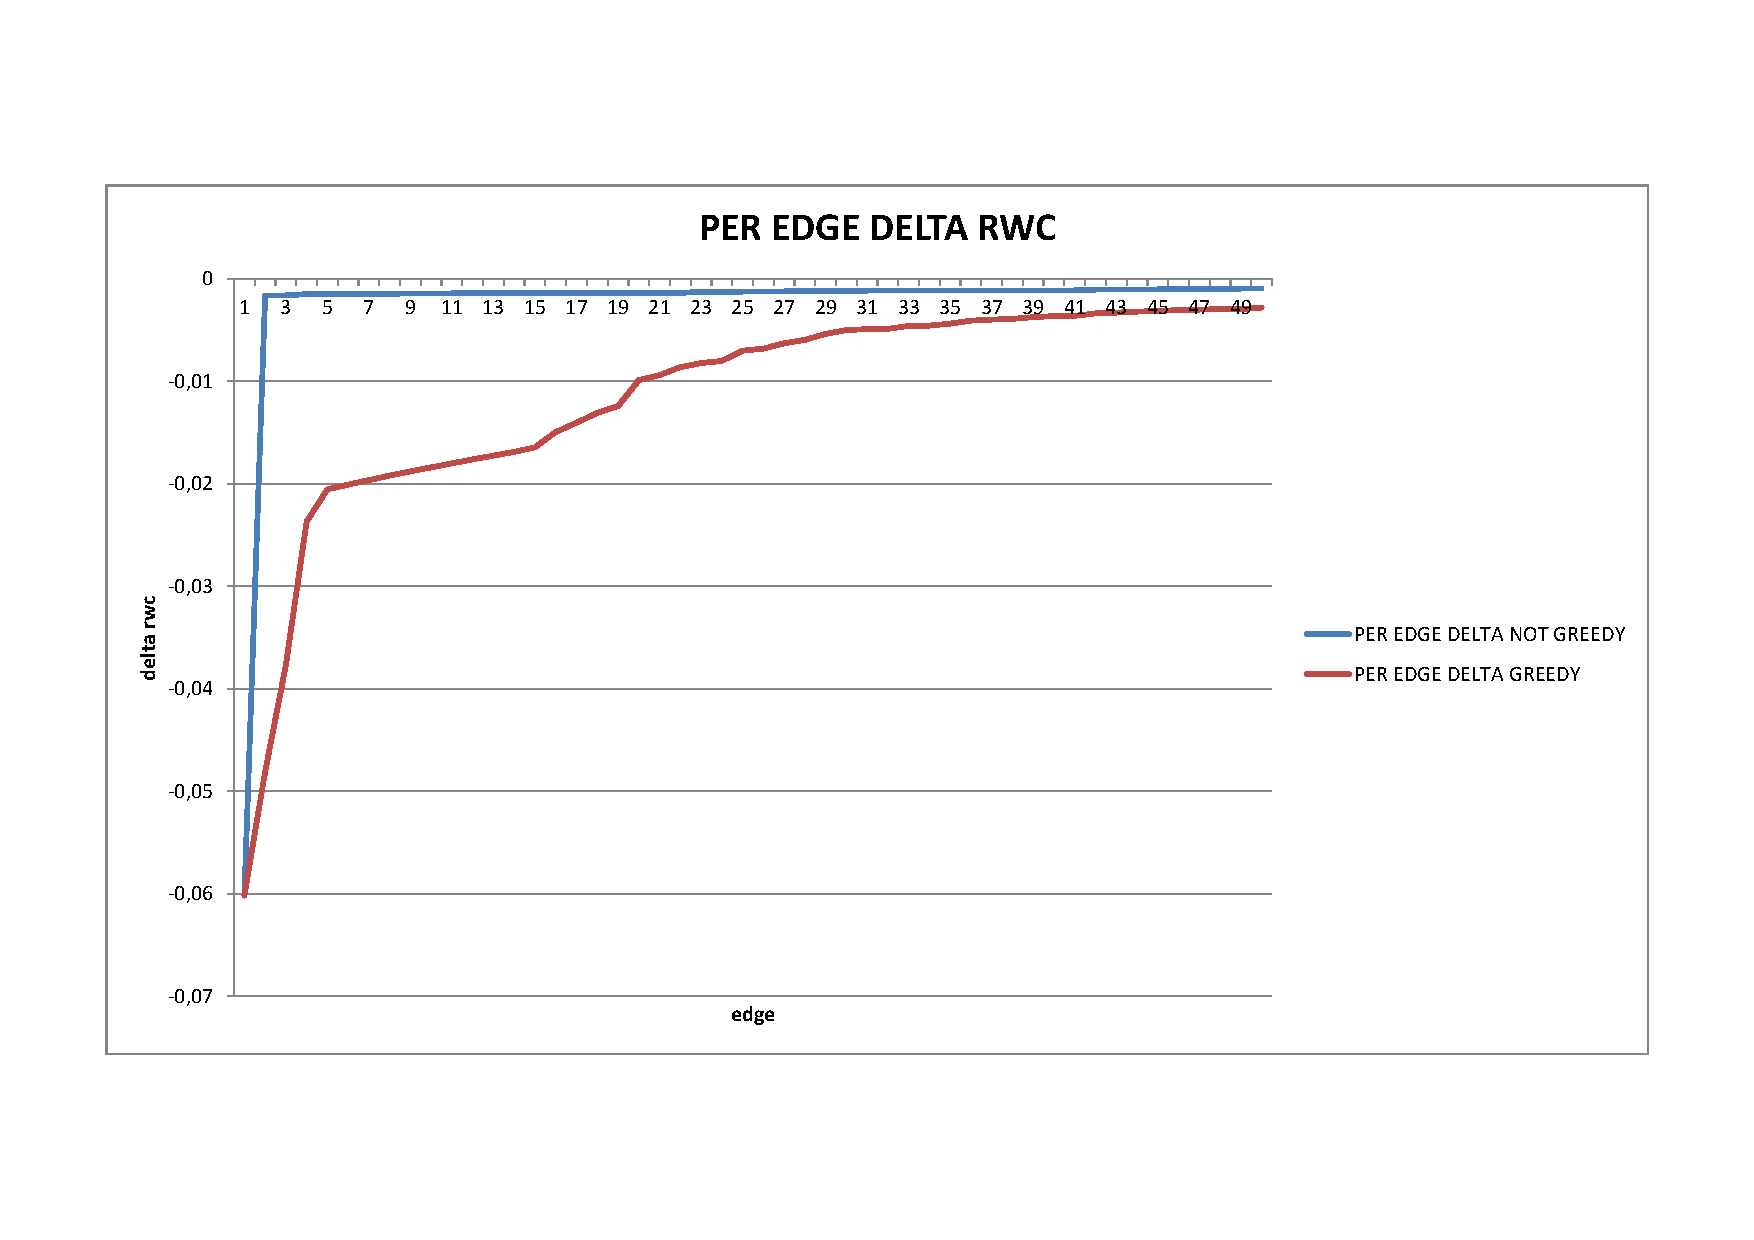
\includepdf{images/INDIANA_IN_DEG_PROBABILITY_FREE_PER_EDGE_DELTA.pdf}
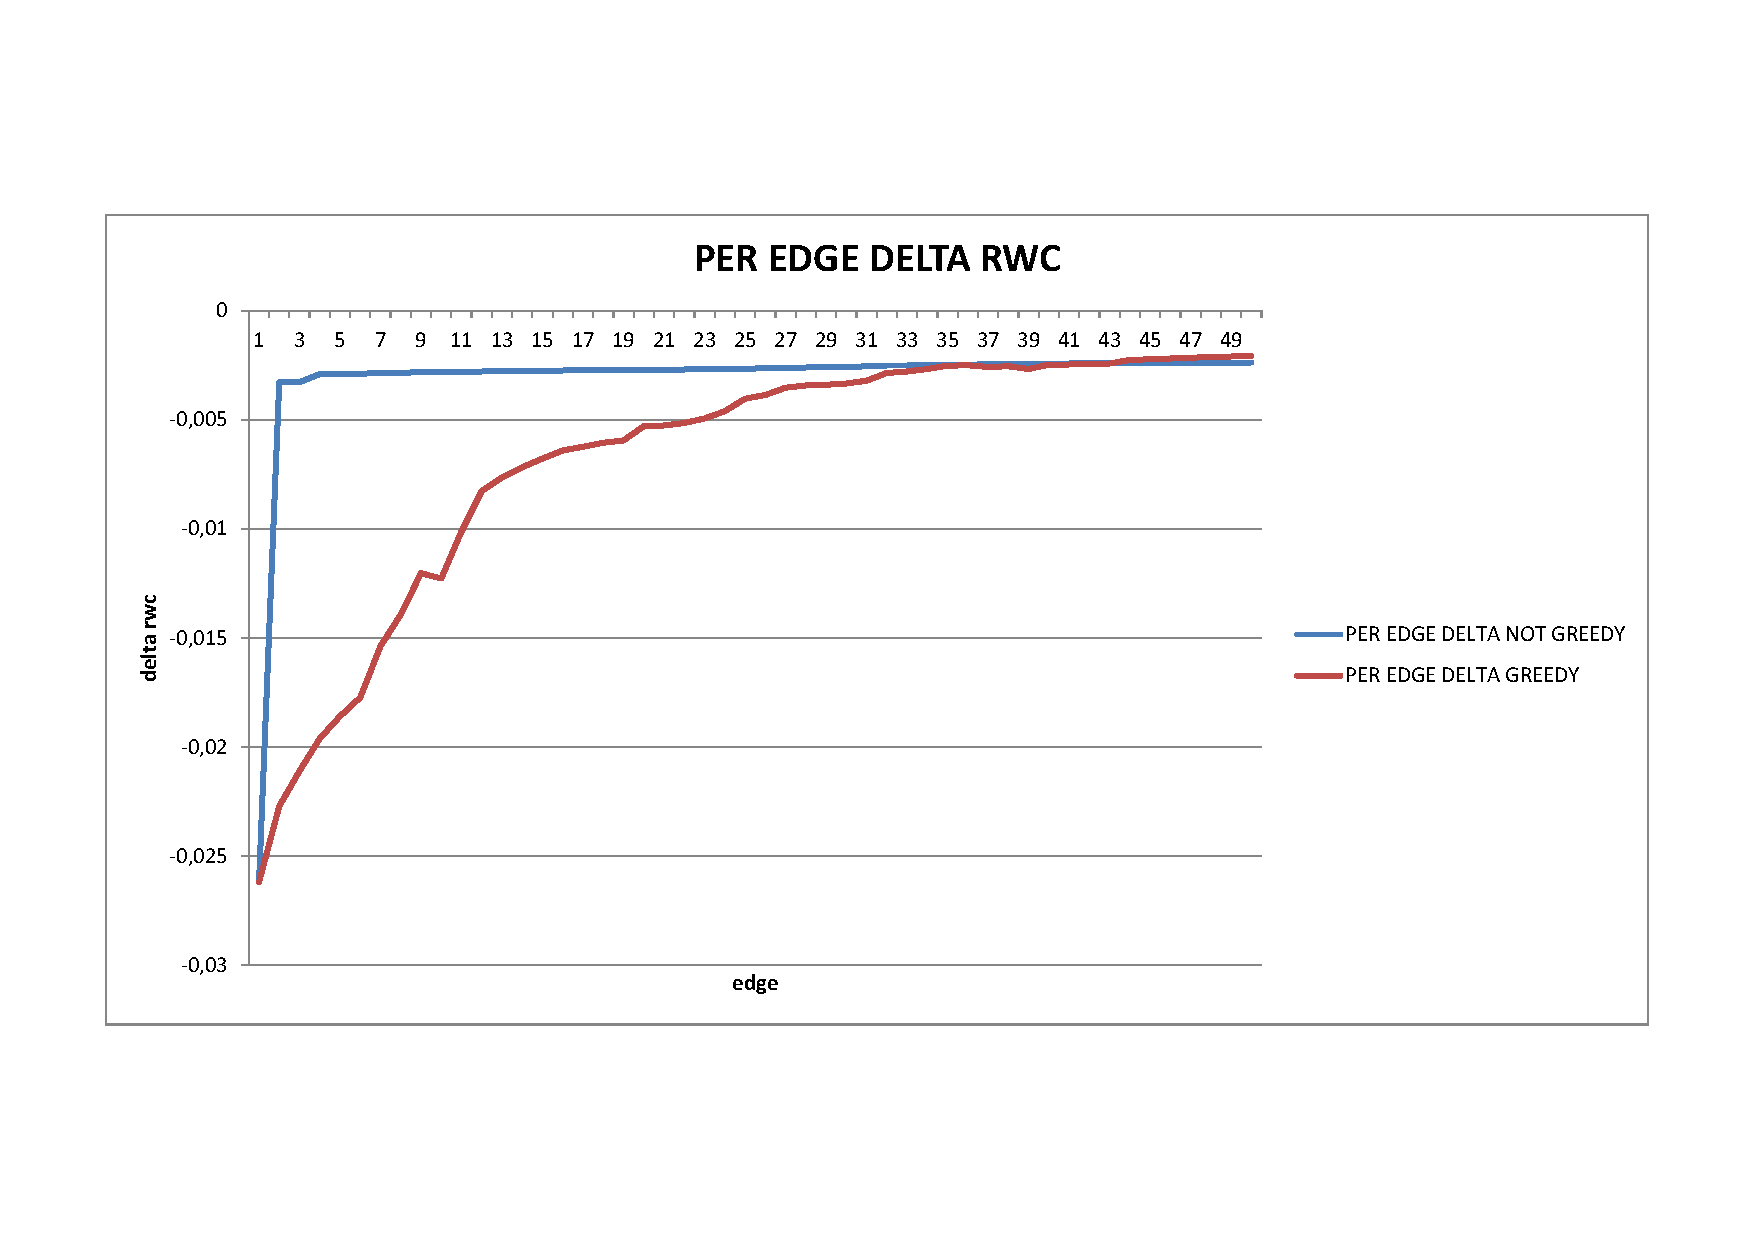
\includepdf{images/RUSSIA_MARCH_IN_DEG_PROBABILITY_FREE_PER_EDGE_DELTA.pdf}
Questa volta ciascuno dei tre grafici, uno per \textit{retweet graph}, ha l'obiettivo di porre a confronto i \textit{$\delta RWC$} associati ai \textit{k} archi che rispettivamente i due algoritmi di \textit{edge recommendation} propongono.
\\Più precisamente, fissato un \textit{retweet graph g}, il grafico corrispondente mostra due funzioni, rispettivamente di colore \textit{rosso} e di colore \textit{blu}, con valori nel dominio \textit{$0 < i \leq k$}\footnote{Ovvero l'\textit{i-esimo} arco proposto.}:
\begin{itemize}
\item \textit{$\delta RWC(g,i)\textsubscript{greedy}$}, ovvero il \textit{$\delta RWC$} che l'\textit{i-esimo} arco proposto dall'algoritmo \textit{greedy} consentirebbe di ottenere qualora si materializzasse successivamente a \textit{tutti} gli archi proposti con indici da \textit{1} a \textit{i-1};
\item \textit{$\delta RWC(g,i)\textsubscript{non-greedy}$}\footnote{Ciascun \textit{$\delta RWC(g,i)\textsubscript{non-greedy}$} non è il \textit{$\delta RWC$} utilizzato dall'algoritmo \textit{non-greedy} come criterio di scelta dell'\textit{i-esimo} arco ma è l'effettivo decremento dell'\textit{RWC} che l'\textit{i-esimo} arco proposto apporterebbe se si materializzasse secondo l'ordine di scelta.}, ovvero il \textit{$\delta RWC$} che l'\textit{i-esimo} arco proposto dall'algoritmo \textit{non-greedy} consentirebbe di ottenere qualora si materializzasse successivamente a \textit{tutti} gli archi proposti con indici da \textit{1} a \textit{i-1}.
\end{itemize}
Anche in questo caso è evidente che, per ogni \textit{retweet graph g} considerato e $\forall i = 1,..,k$, vale:
\\\\
$\textit{$\delta RWC(g,i)\textsubscript{greedy}$} \leq \textit{$\delta RWC(g,i)\textsubscript{non-greedy}$}$
\\\\
Ovvero, nell'ipotesi che tutti gli archi precedentemente proposti vengano accettati, il \textit{$\delta RWC$} associato all'\textit{i-esimo} arco proposto dall'algoritmo \textit{greedy} è minore o uguale al \textit{$\delta RWC$} associato all'\textit{i-esimo} arco proposto dall'algoritmo \textit{non-greedy}, $\forall i = 1,..,k$. Quest'osservazione implica che, generalmente, gli archi scelti da \textit{greedy} sono migliori \textit{qualitativamente} rispetto a quelli scelti da \textit{non-greedy}, poiché determinano un maggior decremento dell'\textit{RWC} associato al \textit{retweet graph} in input.
\\I risultati sinora ottenuti derivano senz'altro dalla maggior precisione del criterio di scelta degli archi dell'algoritmo \textit{greedy} rispetto a quello dell'algoritmo \textit{non-greedy}. 
\\A tal proposito, è possibile utilizzare il \textit{tool di visualizzazione} introdotto nel capitolo precedente per analizzare, per ogni \textit{retweet graph} in input, le caratteristiche dei \textit{k} archi scelti da ciascuno dei due algoritmi e dei nodi coinvolti: quest'analisi potrebbe chiarire ulteriormente le cause che rendono un algoritmo più efficace dell'altro. 
\\A fine capitolo inseriamo gli \textit{outputs} del \textit{tool}, ciascuno dei quali descrive i risultati dell'applicazione di uno dei due algoritmi di \textit{edge recommendation} su un \textit{retweet graph} in input.
\\
Con riferimento alle figure da \ref{fig:beefgreedy} a \ref{fig:russianotgreedy}, si nota che generalmente i \textit{k} archi scelti dall'algoritmo \textit{non greedy} tendono a formare una struttura a \textit{stella}: infatti la maggior parte di essi condivide uno stesso nodo \textit{endpoint}. Ciò è dovuto al fatto che l'algoritmo \textit{non greedy} utilizza come metrica di scelta degli archi il \textit{$\delta RWC$} che ciascuno di essi apporterebbe se fosse aggiunto \textit{individualmente} al grafo, ignorando la potenziale diminuzione dell'efficacia individuale causata dalla loro interazione reciproca. In generale, si osserva che maggiore è la tendenza degli archi scelti a condividere uno stesso \textit{endpoint} e minore è il decremento dell'\textit{RWC} che collettivamente riescono ad apportare: questo è il caso degli archi proposti dall'algoritmo \textit{non greedy} e determina il suo \textit{deficit} di efficacia. 
\section{Tempi di esecuzione}
Questo paragrafo ha lo scopo di mostrare e commentare i tempi di esecuzione dei due algoritmi di \textit{k-edge recommendation}, espressi in funzione del \textit{retweet graph} in input. Si consideri la seguente tabella:
\\\\
\begin{tabular}{l*{6}{c}r}
\textbf{Hashtag}         & \textbf{greedy} & \textbf{non greedy}  \\
\hline
\#beefban 		 & 7252 sec & 159 sec  \\
\#indiana        	 & 17580 sec & 372 sec \\
\#russia\_march   	 & 12720 sec & 293 sec  \\
\end{tabular}
\\\\\\

\begin{figure}
\begin{center}
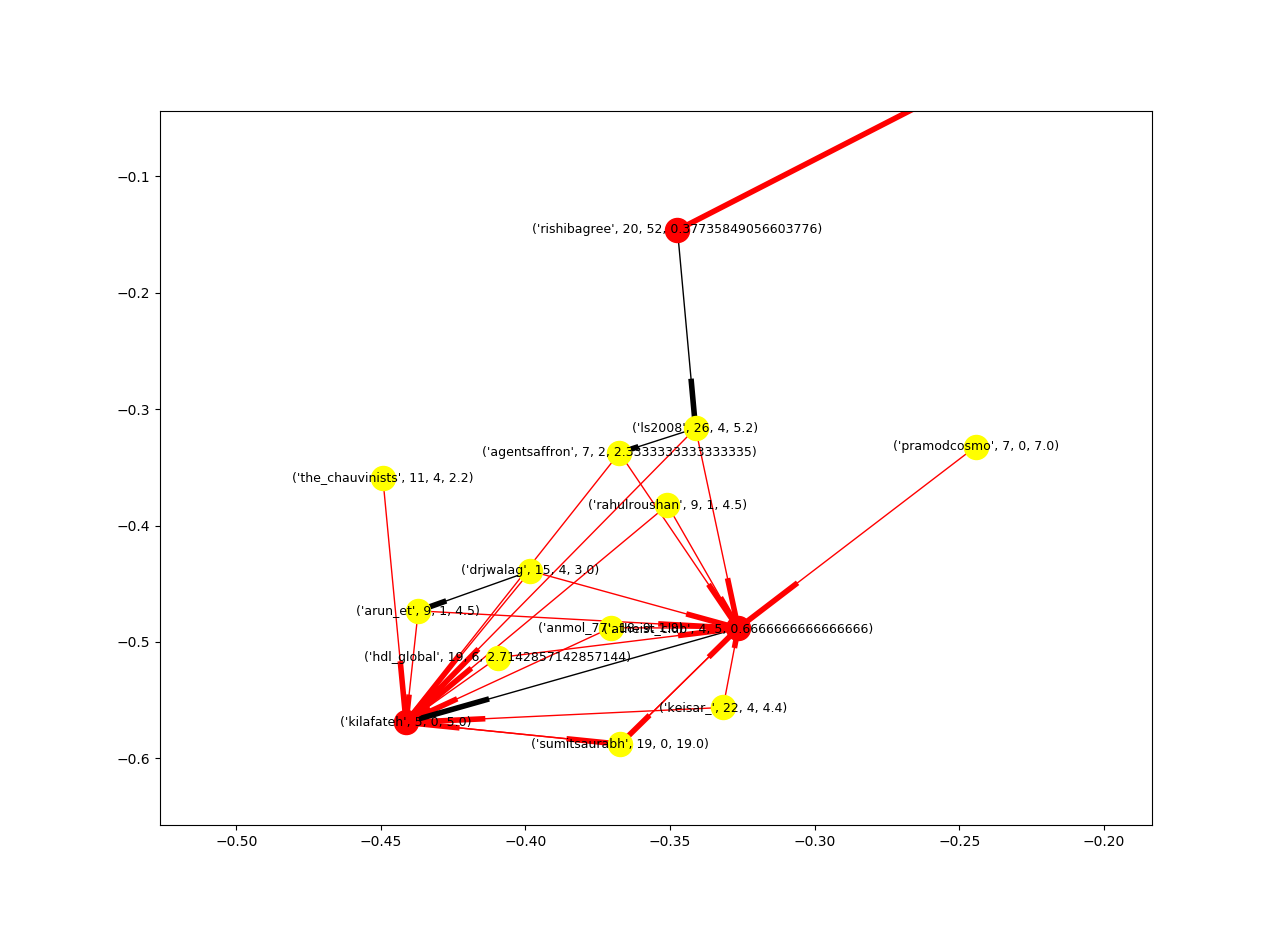
\includegraphics[scale=0.5]{images/beefban_in_degree_greedy_probability_free.png}
\end{center}
\caption{Porzione dell'\textit{output} del \textit{tool} a seguito dell'esecuzione di \textit{greedy} sul \textit{retweet graph \#beefban}.}
\label{fig:beefgreedy}
\end{figure}

\begin{figure}
\begin{center}
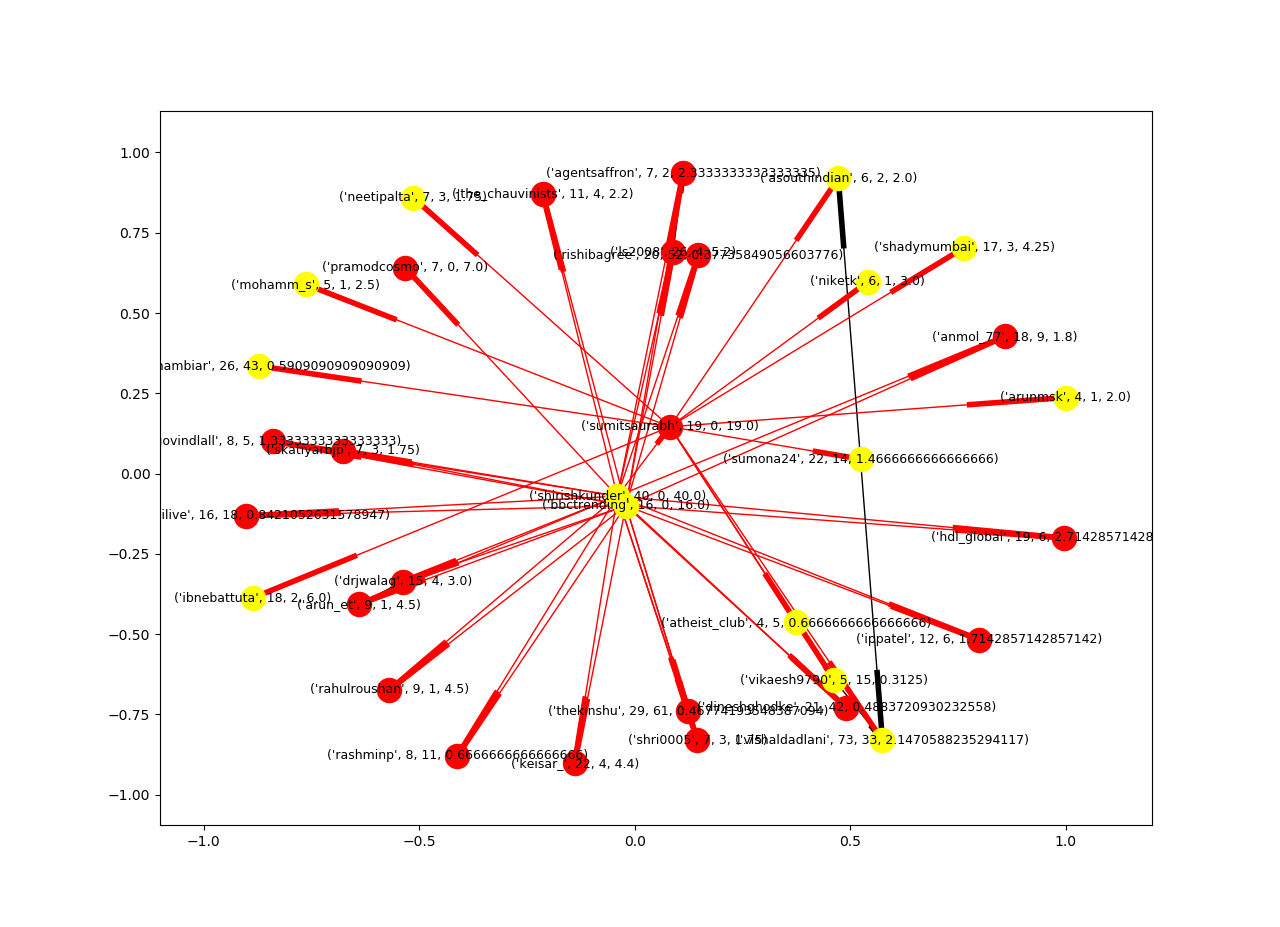
\includegraphics[scale=0.5]{images/beefban_in_degree_probability_free.png}
\end{center}
\caption{Porzione dell'\textit{output} del \textit{tool} a seguito dell'esecuzione di \textit{non greedy} sul \textit{retweet graph \#beefban}.}
\label{fig:beefnotgreedy}
\end{figure}

\begin{figure}
\begin{center}
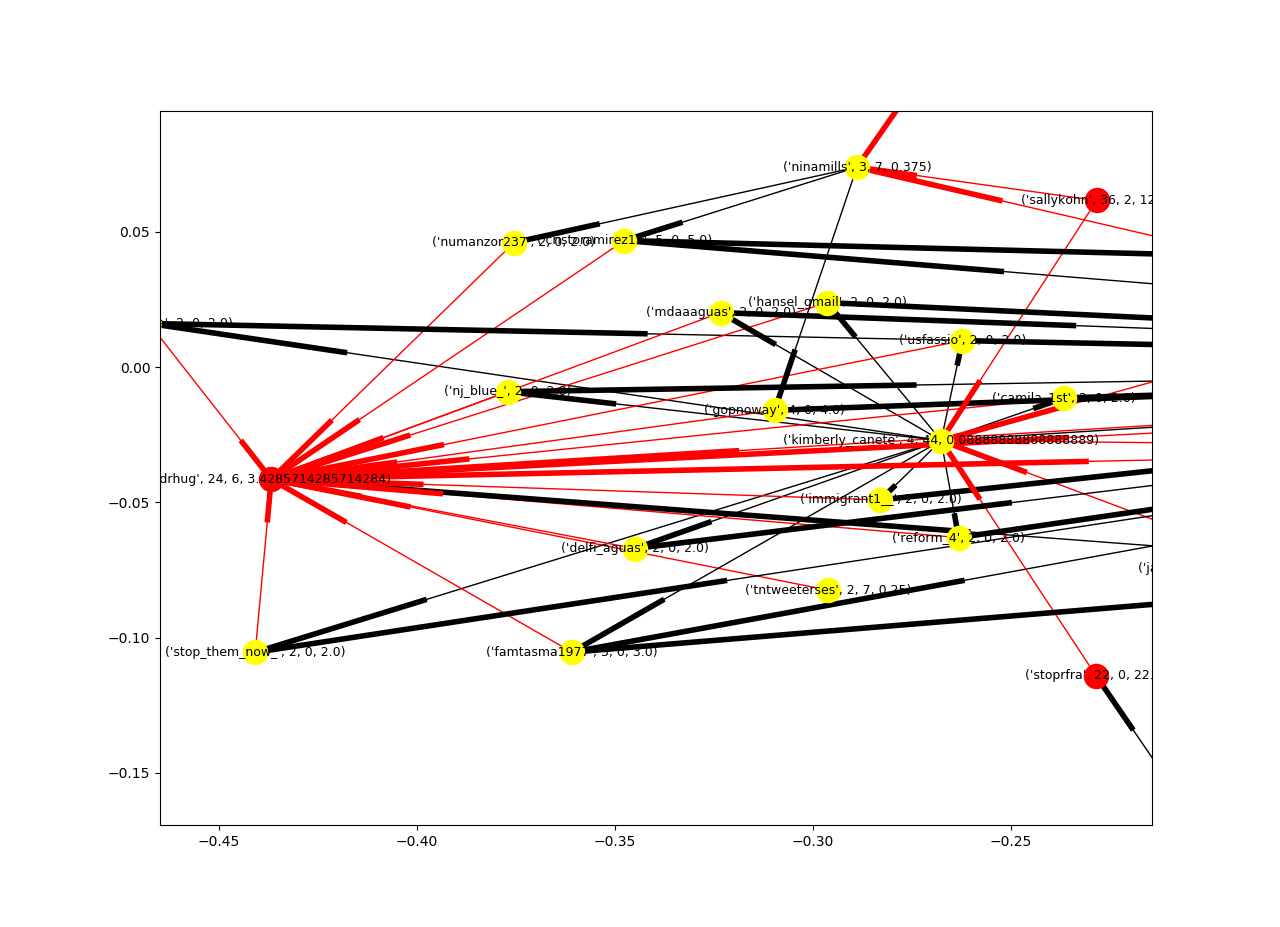
\includegraphics[scale=0.5]{images/indiana_in_degree_greedy_probability_free.png}
\end{center}
\caption{Porzione dell'\textit{output} del \textit{tool} a seguito dell'esecuzione di \textit{greedy} sul \textit{retweet graph \#indiana}.}
\label{fig:indigreedy}
\end{figure}

\begin{figure}
\begin{center}
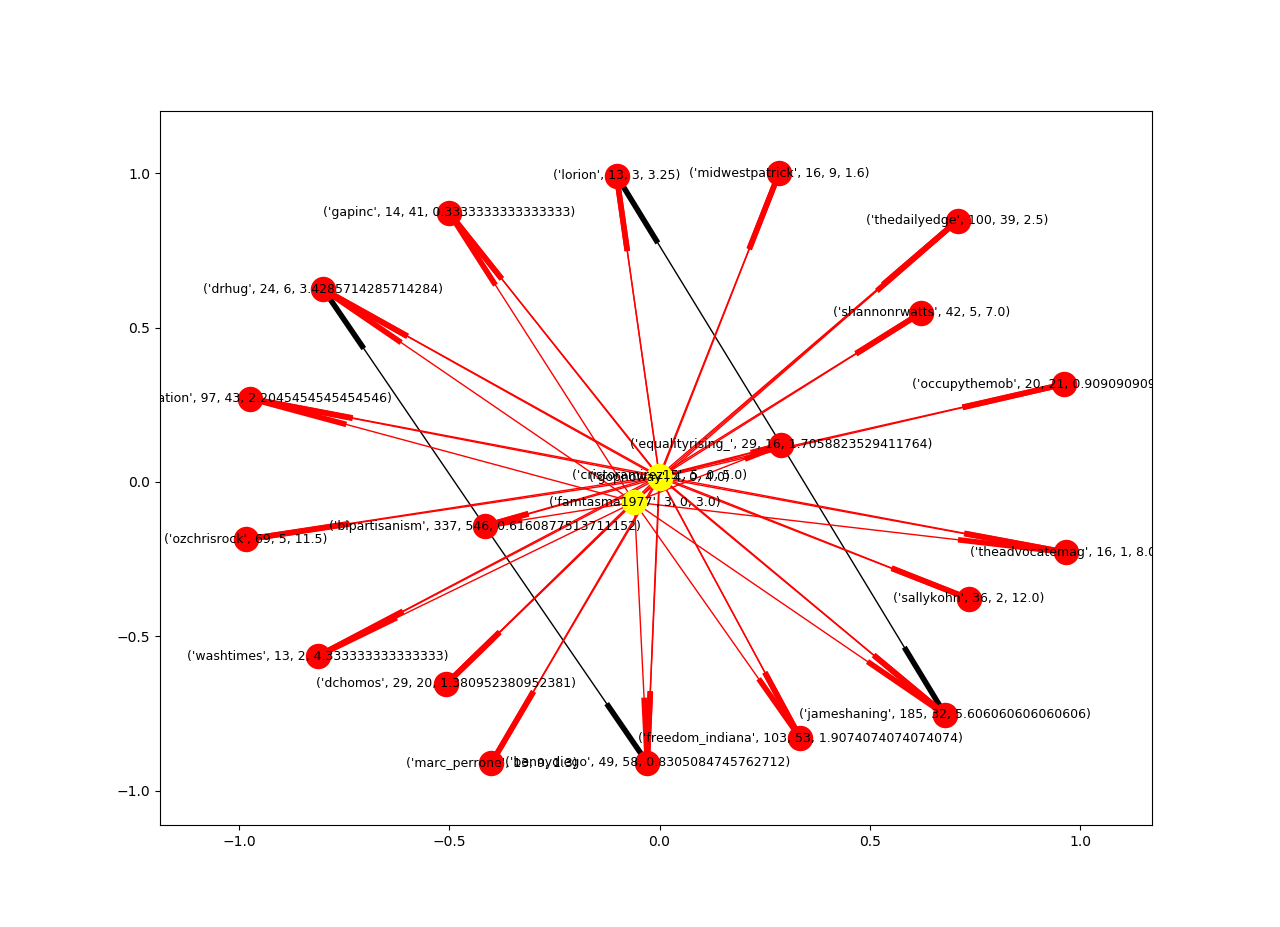
\includegraphics[scale=0.5]{images/indiana_in_degree_probability_free.png}
\end{center}
\caption{Porzione dell'\textit{output} del \textit{tool} a seguito dell'esecuzione di \textit{non greedy} sul \textit{retweet graph \#indiana}.}
\label{fig:indinotgreedy}
\end{figure}

\begin{figure}
\begin{center}
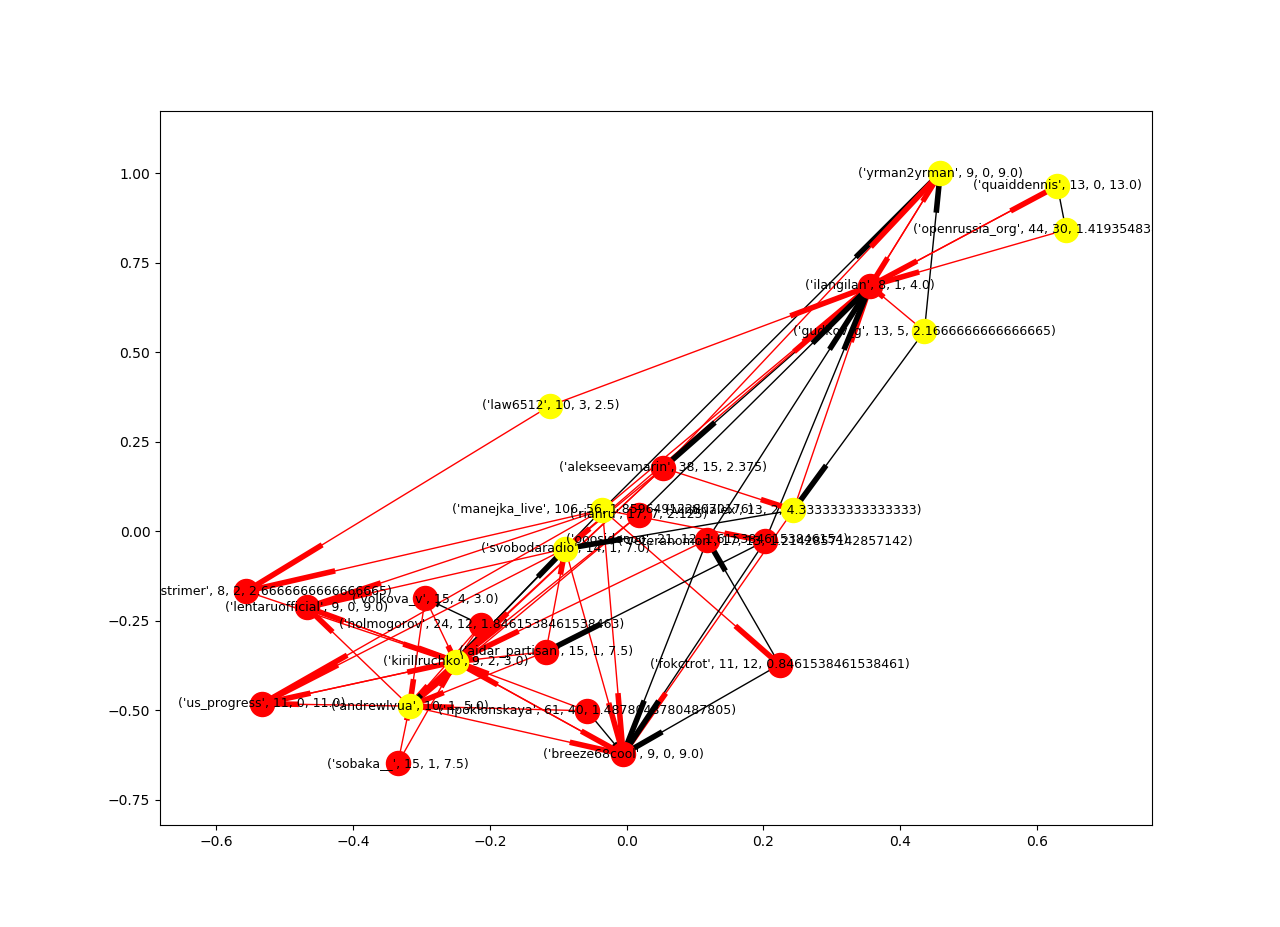
\includegraphics[scale=0.5]{images/russia_march_in_degree_greedy_probability_free.png}
\end{center}
\caption{Porzione dell'\textit{output} del \textit{tool} a seguito dell'esecuzione di \textit{greedy} sul \textit{retweet graph \#russia\_march}.}
\label{fig:russiagreedy}
\end{figure}

\begin{figure}
\begin{center}
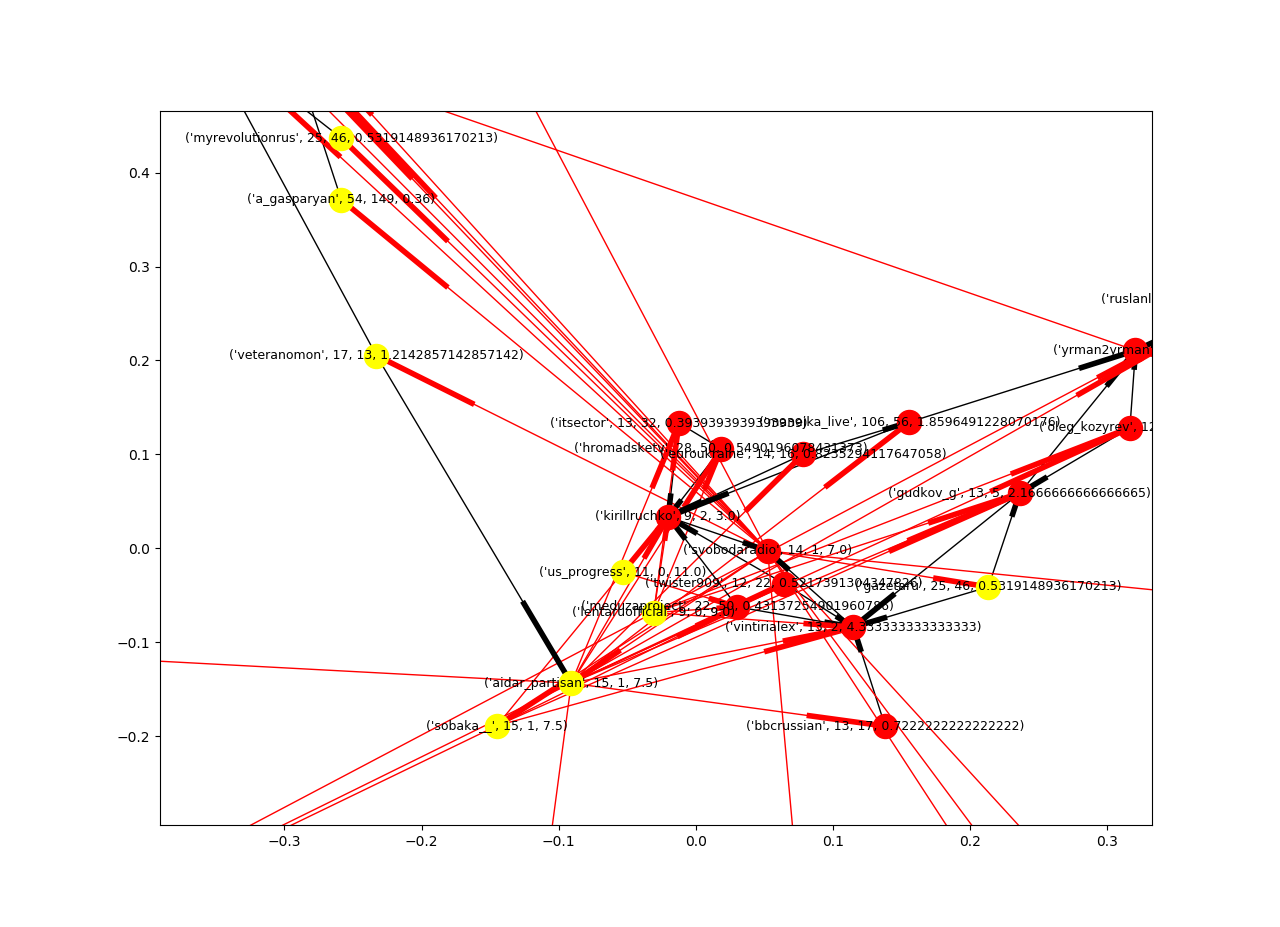
\includegraphics[scale=0.5]{images/russia_march_in_degree_probability_free.png}
\end{center}
\caption{Porzione dell'\textit{output} del \textit{tool} a seguito dell'esecuzione di \textit{non greedy} sul \textit{retweet graph \#russia\_march}.}
\label{fig:russianotgreedy}
\end{figure}



